

Cette option s'annule  lorsque la barrière est franchie, elle est considerée comme exotique. Elle est une option plus sûre pour le vendeur car elle met une limite aux pertes potentiellement infinies sinon. Comme c'est une option plus risquée pour l'acheteur le prix de l'option est inférieur à celui d'une option vanille traditionelle. On la connait comme un CALL {\slshape up and out}. De plus on modelisera aussi un PUT avec barrière pour comprendre, comment implémenter la barrière et avoir une vision globale sur les 2 options. Le PUT avec barrière, aussi connu comme PUT {\slshape down and out} possède un barrière inférieure. On fera l'analyse avec une barrière à 65. Les Figure~\ref{fig:put_bar_payoff} et Figure~\ref{fig:call_bar_payoff} représentant le payoff de cette option en $t=T$ en fonction du cours du sous-jacent, $S_t$.

\begin{figure}[H]
\centering
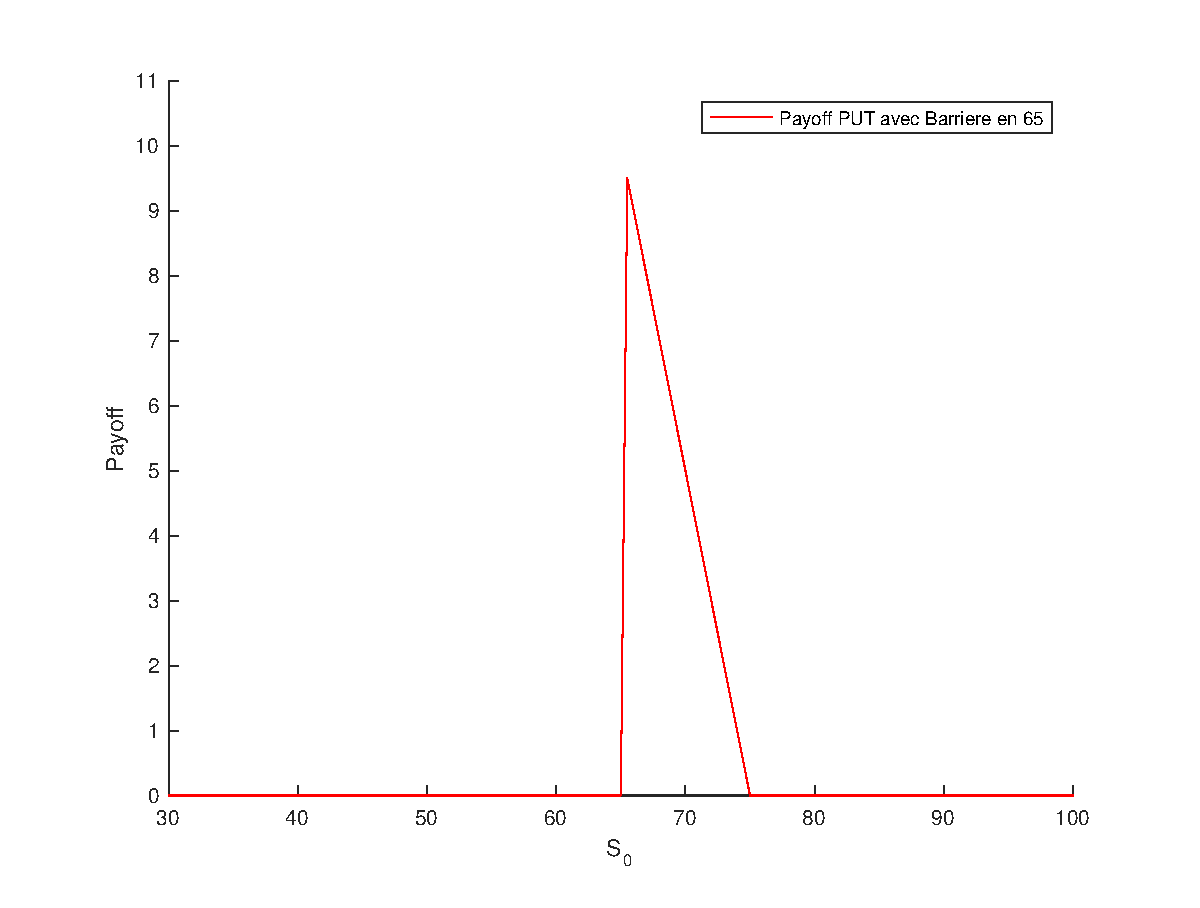
\includegraphics[scale=0.5]{./img/PUT_BAR_PAYOFF.eps}
\caption{Payoff d'une option barrière sur un PUT européen  en fonction du cours du sous-jacent}
\label{fig:put_bar_payoff}
\end{figure}

\begin{figure}[H]
\centering
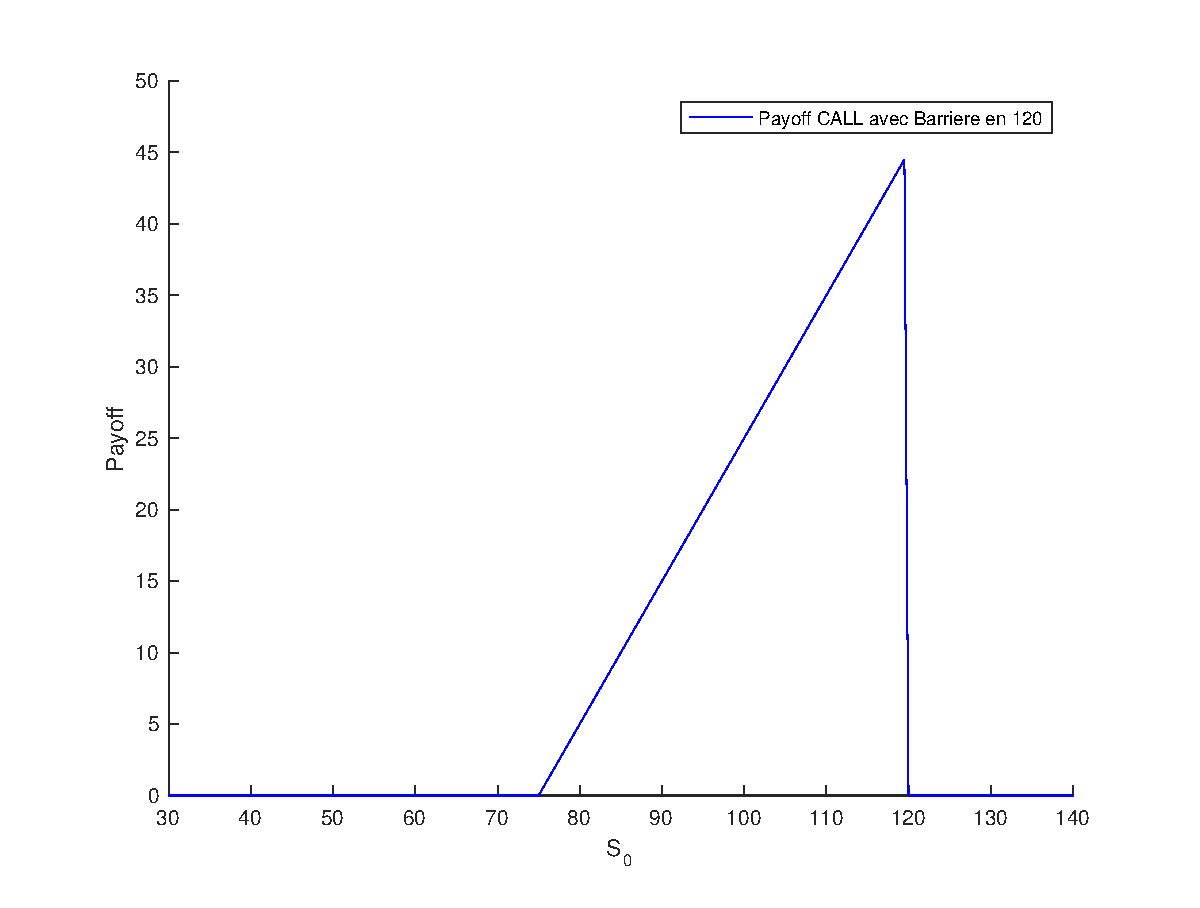
\includegraphics[scale=0.5]{./img/CALL_BAR_PAYOFF.eps}
\caption{Payoff d'une option barrière sur un CALL européen  en fonction du cours du sous-jacent}
\label{fig:call_bar_payoff}
\end{figure}

\subsection{Méthode de Monte-Carlo} % (fold)

\label{sub:methode_de_monte_carlo}

On analyse le prix de l'option en réalisant l'approximation de Monte-Carlo. La fonction pour le réaliser est Listing~\ref{listing:7}, le fichier dans lequel on la implémentée est \textsc{option$\_$barriere.py}. Les Figure~\ref{fig:call_put__bar_mc_tir}, Figure~\ref{fig:call_put_bar_mc} présentent les résultats obtenus.

\begin{figure}[H]
\centering
\includegraphics[scale=0.6]{./img/CALL_PUT_BAR_MC_TIR.eps}
\caption{Variation d'une option européenne avec option barrière approché par la méthode de Monte-Carlo en fonction du nombre de tirages}
\label{fig:call_put__bar_mc_tir}
\end{figure}

\begin{figure}[H]
\centering
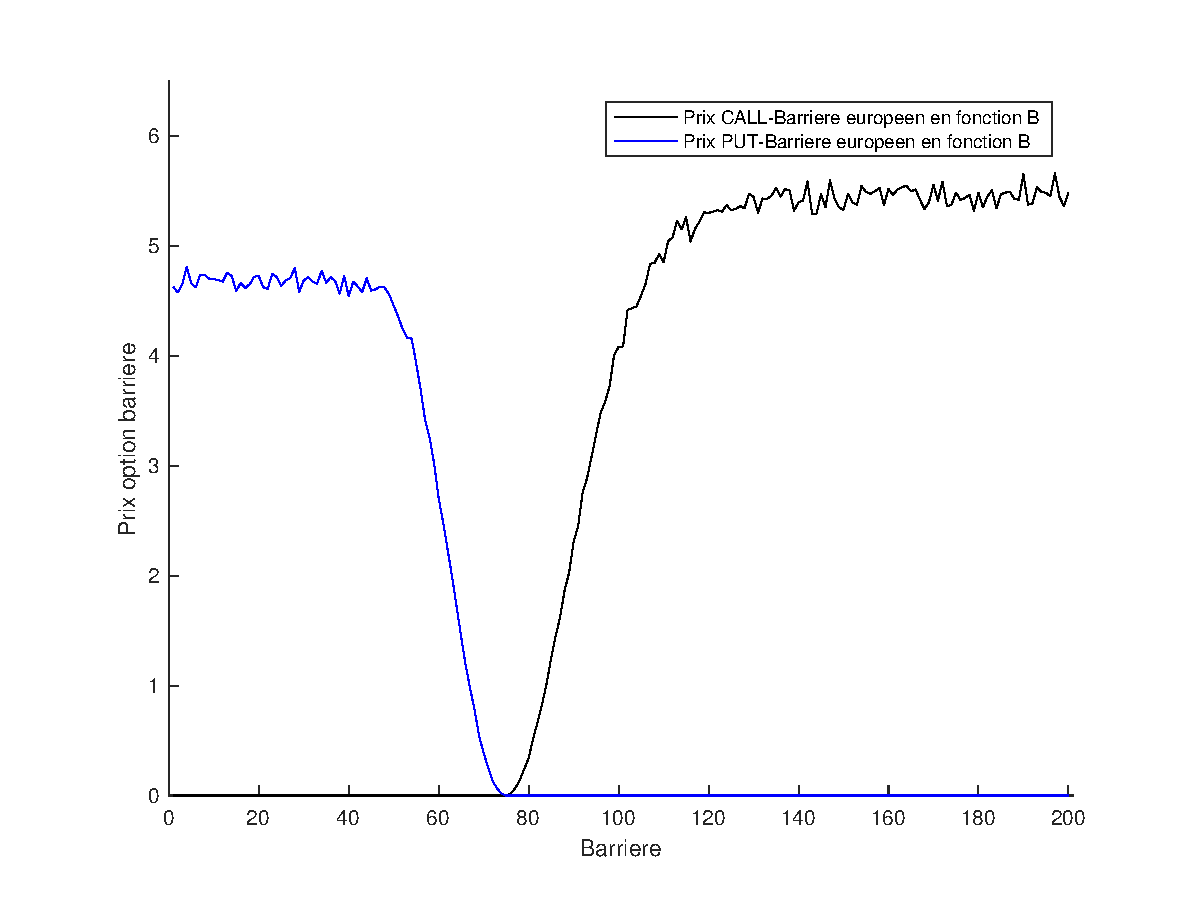
\includegraphics[scale=0.6]{./img/CALL_PUT_BAR.eps}
\caption{Variation d'une option européenne avec option barrière approché par la méthode de Monte-Carlo en fonction du niveau de la barrière}
\label{fig:call_put_bar_mc}
\end{figure}
% subsection methode_de_monte_carlo (end)

On peut voir que le prix du CALL augmente avec le niveau de la barriere et pour un barriere très grande, le prix est celui du modèle Black and Scholes. Pour le Put c'est exactement le contraire. Ce qui est logique, en effet si on pose la barrière très en dessous du prix \emph{At the Money} dans le cas d'un CALL, il est presque impossible que l'on ai un gain. Un raisonement similaire peut se faire pour le PUT.

On voit que le prix du PUT est inferieur au prix du CALL, car l'espérance de gain est inférieure.

\newpage

\subsection{Modèle Binomial} % (fold)
\label{sub:modele_binomial}

On analyse le prix de l'option dans le cadre du modèle binomial. La fonction pour le réaliser est Listing~\ref{listing:8}, le fichier dans lequel on la implémentée est \textsc{option$\_$barriere.py}. Les Figure~\ref{fig:call_put_bar_mb_prof}, Figure~\ref{fig:call_put_bar_mb} présentent les résultats obtenus.


Il est intéressant d'analyser comme sur la Figure~\ref{fig:call_put_bar_mb_prof} il y a plus de variations du PUT. La raison apparait sur la Figure~\ref{fig:call_put_bar_mb}, en effet on peut observer que pour un niveau de la barrière à 65, le delta du PUT est plus élevé que celui du CALL pour un niveau égal à 120.

\begin{figure}[H]
\centering
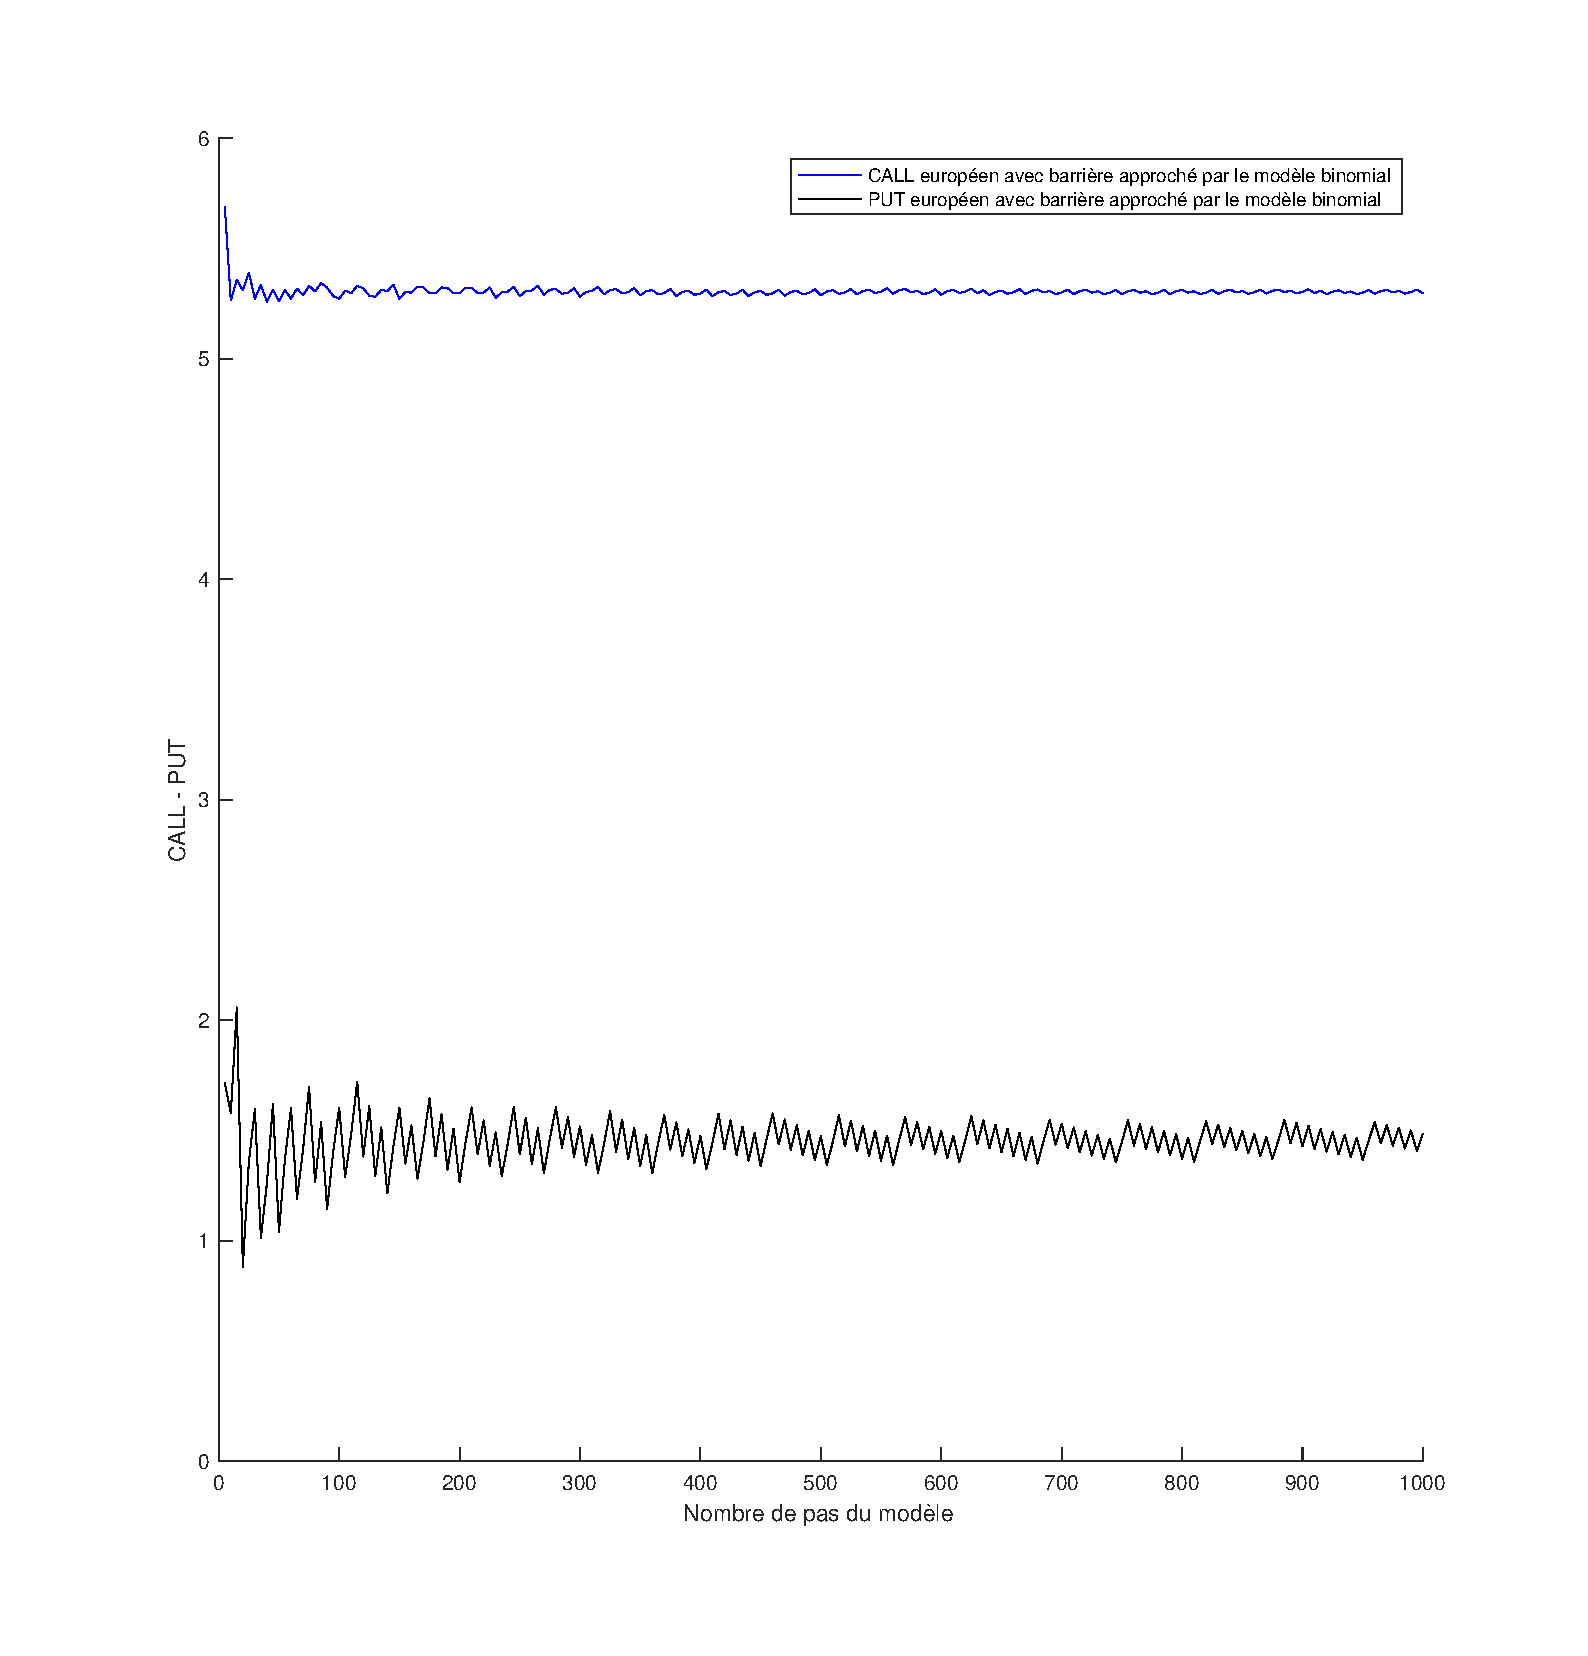
\includegraphics[scale=0.5]{./img/CALL_PUT_BAR_MB_PROFONDEUR.eps}
\caption{Variation d'une option européenne avec option barrière approché par le modèle binomial en fonction du pas}
\label{fig:call_put_bar_mb_prof}
\end{figure}

\begin{figure}[H]
\centering
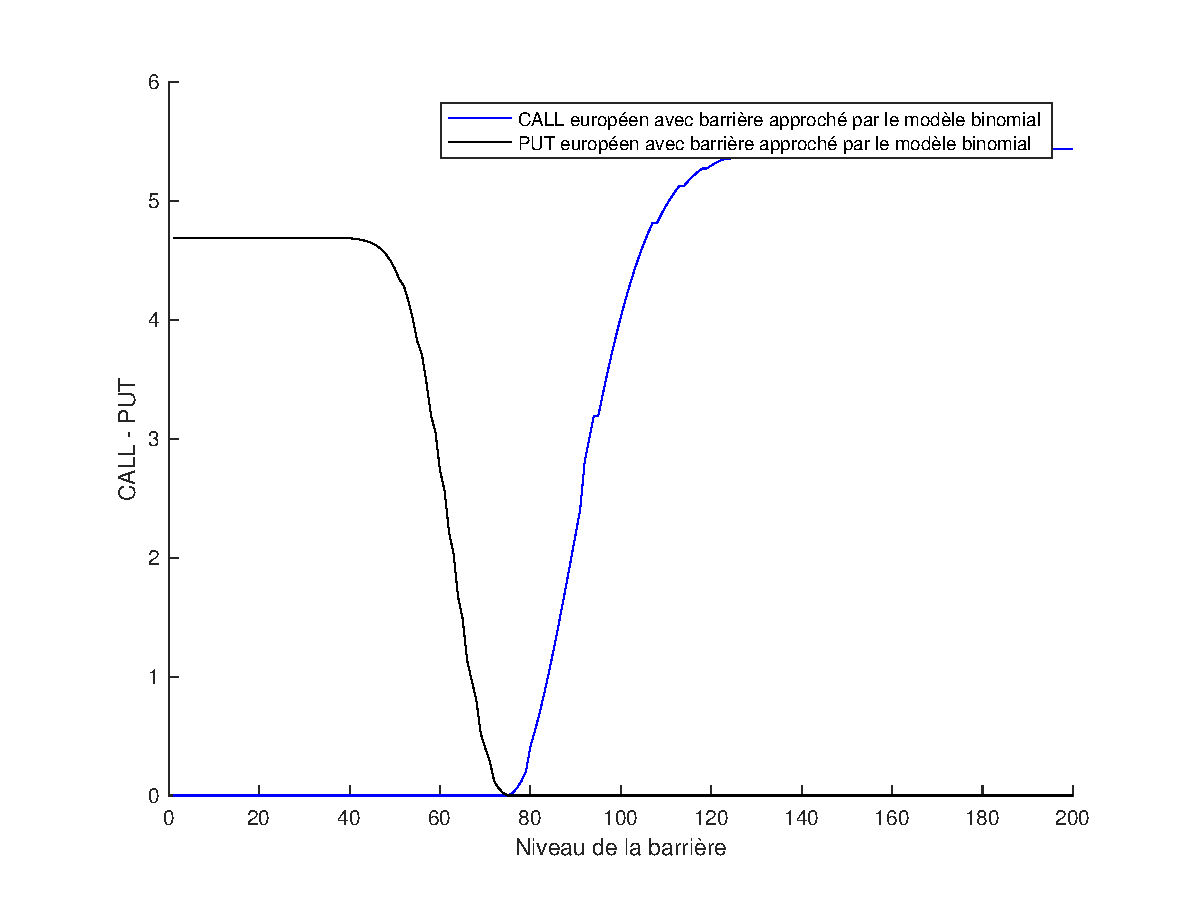
\includegraphics[scale=0.6]{./img/CALL_PUT_MB_BAR.eps}
\caption{Variation d'une option européenne avec option barrière approché par le modèle binomial en fonction du niveau de la barrière}
\label{fig:call_put_bar_mb}
\end{figure}

Les remarques sur les variations en fonction du PUT son les mêmes que dans le cadre Monte-Carlo. De plus on observe un lissage plus important, en effet la méthode de Monte-Carlo nécessite plus de tirages pour obtenir un résultat équivalent au modèle binomial. Cependant le grand avantage de la méthode de Monte-Carlo est que l'on n'a pas besoin de connaitre le modèle pour obtenir des résultats.

% subsection modele_binomial (end)